\begin{center}
  \Large
  \textbf{BIOGRAFI PENULIS}
\end{center}

\addcontentsline{toc}{chapter}{BIOGRAFI PENULIS}

\vspace{2ex}

\begin{wrapfigure}{L}{0.3\textwidth}
  \centering
  \vspace{-3ex}
  % Ubah file gambar berikut dengan file foto dari mahasiswa
  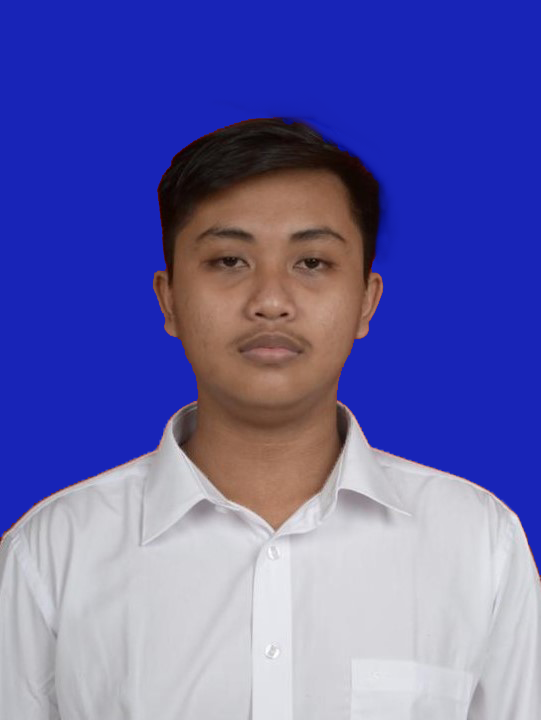
\includegraphics[width=0.3\textwidth]{BiografiPenulis/BG BIRU.png}
  \vspace{-4ex}
\end{wrapfigure}

% Ubah kalimat berikut dengan biografi dari mahasiswa
\name{}, atau yang biasa dikenal sebagai Depa, lahir di Tabanan, Bali pada 8 Februari 2002. Penulis merupakan anak pertama dari dua bersaudara yang tinggal dan tumbuh besar di pedesaan kecil di perbatasan antara Tabanan dan Negara, Bali. Penulis merupakan lulusan SMA Negeri 1 Tabanan dan melanjutkan pendidikan ke jenjang strata satu di Departemen Teknik Komputer Fakultas Teknologi Elektro dan Informatika Cerdas Institut Teknologi Sepuluh Nopember (ITS) pada tahun 2021.

Selama masa studinya, penulis menunjukkan minat yang kuat dalam bidang teknologi, terutama pada pengembangan kecerdasan buatan, dan \emph{machine learning}. Ketertarikan ini mendorongnya untuk mendalami topik-topik seperti \emph{machine learning} dan \emph{Internet of Things} (IoT).

Pada penelitian tugas akhir ini, penulis memilih mengembangkan sistem kendali kursi roda berbasis SIBI dan memiliki sistem pengereman otomatis agak meminimalisir kecelakaan.
